\documentclass{article}
\usepackage{tikz, comment}
\usepackage{pifont}
\usepackage{fontspec, pgfplots}
\usetikzlibrary{arrows, decorations.markings, decorations.pathreplacing}
\begin{comment}
:Title: Not defined yet
:Tags: parabola;moment;focus of a parabola;focal radius ;dimensions
:Prob: 0.4875;0.4815;0.4786;0.4734;0.4719
:Author: Prof.Hu Ji-shan, HKUST
:Slug: No name yet

Description Here.........
\end{comment}
\begin{document}\centering 

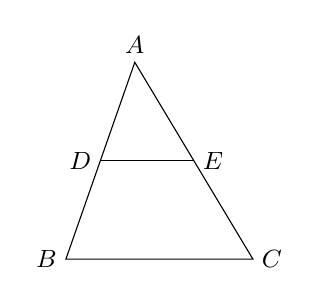
\begin{tikzpicture}[>=latex,xscale=.5*5, yscale=.5*5][font=\sf\small] 

\draw (0, 0)node[above]{$A$} -- (-0.35, -1)node[left]{$B$} -- (0.6, -1)node[right]{$C$} -- cycle;

\draw ({-0.35/2}, {-1/2})node[left]{$D$} -- ({0.6/2}, {-1/2})node[right]{$E$};

\end{tikzpicture}
\end{document}